\newpage
\section{Introduction to QRobots}
\labelsec{introQRobots}
 
Since a \texttt{QRobot} (see \xs{QRobot} ) is a \texttt{QActor} able to interact with an instance of a \textit{BaseRobot}, we must first of all understand what is a \textit{BaseRobot}.
%%, as shown in the following picture:

%% \begin{center}
%%\begin{tabular}{ c }
%%     \includegraphics[scale = 0.65]{../../../it.unibo.iss2015intro/docs/Robots/robotActor.jpg}\\
%%\end{tabular} 
%%\end{center}

\medskip 
From the physical point of view, a \texttt{BaseRobot} is a custom device built with low-costs components including sensors, actuators and processing units like \textit{RaspberryPi} and \textit{Arduino}. Examples are given in the following picture:

\begin{center}
\begin{tabular}{ c }
     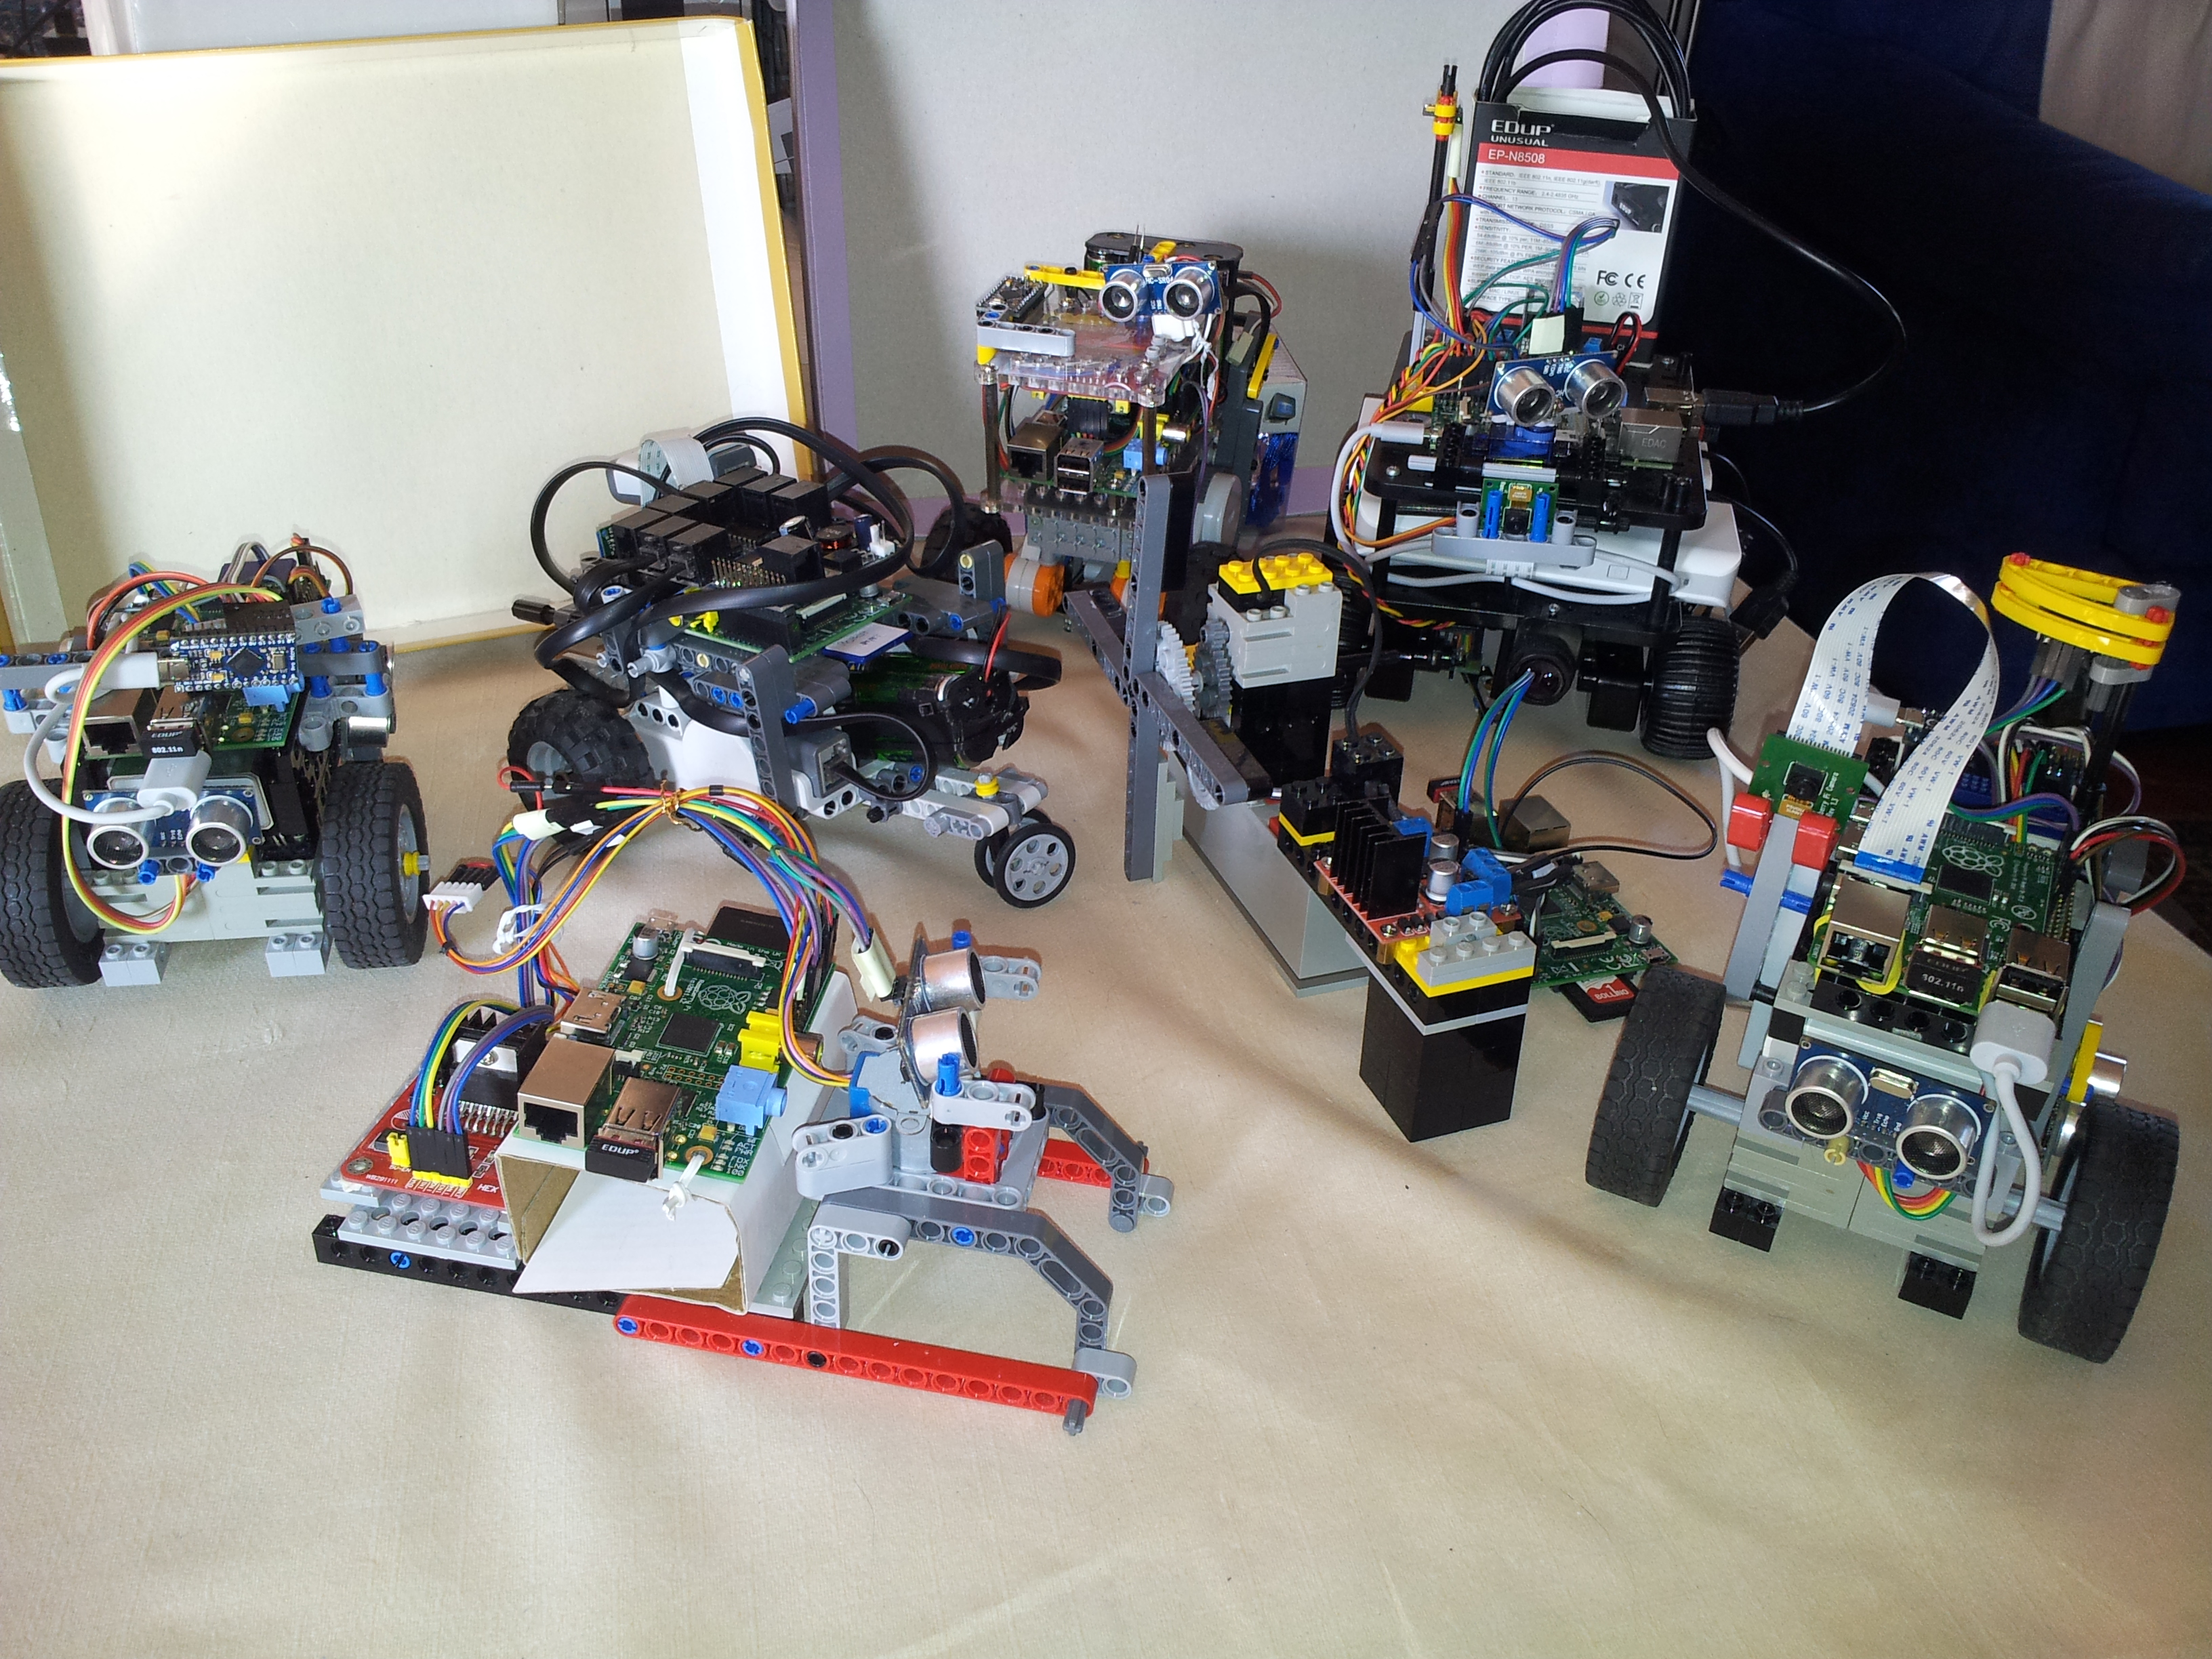
\includegraphics[scale = 0.09]{../../../it.unibo.iss2015intro/docs/imgs/robot/customDevs.jpg}\\
\end{tabular} 
\end{center}


The hardware components of a \texttt{BaseRobot} and their configuration can be quite different from robot to robot. Thus, some software layer is required to hide these differences as much as possible and to build a 'technology independent' layer, to be used by application designers.

A software layer of this kind is provided by the library \textit{labbaseRobotSam.jar}. More specifically:  


\medskip 
\noindent 
\begin{tabular}{|p{0.30\textwidth}|p{0.70\textwidth}|}
\hline 
\textit{it.unibo.lab.baseRobot } 
&The basic software for differential drive robots that are able to move and to acquire sensor data. 

\medskip 
Library: \textit{labbaseRobotSam.jar}. 
\\ 
\hline 
\textit{it.unibo.lab.baseRobot.example} 
&Example of the usage of the \texttt{API} of a BaseRobot.
\\ 
\hline 
\end{tabular} 


\subsection{A model for the BaseRobot}
\labelssec{BaseRobotModel}

The main goal of the \textit{labbaseRobotSam.jar} library is to simplify the work of an application designer by exposing at application level a very simple model of a \texttt{BaseRobot}:

\begin{itemize}
\item As regards the \textbf{\textit{structure}}, a \texttt{BaseRobot} can be viewed as a entity composed of two main parts:
\begin{itemize}
\item An executor (with interface \texttt{IBaseRobot}), able to move the robot according to a  a prefixed set of movement commands (\texttt{IBaseRobotCommand}) 
\item A set of GOF-observable sensors (each with interface \texttt{ISensor}), each working as an active source of data.
\end{itemize}
\item As regards the \textbf{\textit{interaction}}, a \texttt{BaseRobot} can be viewed as a POJO that implements the interface \texttt{IBaseRobot}, while providing a (possibly empty) set of observable sensors;
\item  As regards the \textbf{\textit{behavior}}, a \texttt{BaseRobot} is an object able to execute \texttt{IBaseRobotCommand} and able to update sensor observers defined by the application designer.
\end{itemize}


\begin{center}
\begin{tabular}{ c }
     \includegraphics[scale = 0.8]{../../../it.unibo.lab.baseRobot/umlModels/BasicRobot.jpg}\\
\end{tabular} 
\end{center}

The interface \texttt{IBasicRobot} is introduced as a (GOF) \textit{Facade} for the model.
\lstinputlisting[language=java,caption={ \texttt{IBasicRobot.java} }, firstline=1  ]{../../../it.unibo.lab.baseRobot/src/it/unibo/iot/baseRobot/hlmodel/IBasicRobot.java}

\subsection{The BasicRobot class}
\labelssec{BasicRobot}

The class \texttt{BasicRobot} provides a factory method to create a \texttt{BaseRobot} and to select its main components.

\lstinputlisting[language=java,caption={ \texttt{BasicRobot.java} }, firstline=1  ]{../../../it.unibo.lab.baseRobot/src/it/unibo/iot/baseRobot/hlmodel/BasicRobot.java}

This class shows that the work to set-up and access to the internal structure of a \texttt{BaseRobot} is delegated to a  \texttt{Configurator}. This Configurator reads the specification of the robot structure written in a file named \textit{iotRobot.properties}.   



\subsection{Using a BaseRobot}
\labelssec{}

Let us introduce (project \textit{it.unibo.lab.baseRobot.example}) a robot with configuration named \texttt{\textbf{mocksimple}}, equipped with two motors and a distance sensor, all simulated. 

\subsubsection{The project workspace}
\labelssec{workspace}

The application designer must organize its project workspace as shown in the following snapshot:

\begin{center}
\begin{tabular}{ c }
     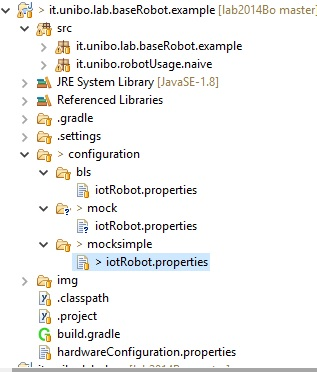
\includegraphics[scale = 0.7]{./img/baseRobotProject.jpg}\\
\end{tabular} 
\end{center}

\subsubsection{The code}
\labelssec{workspace}

The application: \textit{i)} first creates a sensor observer and adds it to all the sensors; \textit{ii)} then it tells the robot to execute the commands it is able to understand.

\lstinputlisting[language=java,caption={ \texttt{BasicRobotUsageNaive.java} }, firstline=1  ]{../../../it.unibo.lab.baseRobot.example/src/it/unibo/robotUsage/naive/BasicRobotUsageNaive.java}

\begin{center}
\begin{tabular}{ c }
     \includegraphics[scale = 0.7]{../../../it.unibo.lab.baseRobot/umlModels/CommandModel.jpg}\\
\end{tabular} 
\end{center}

\subsection{The work of the Configurator}
\labelssec{Configurator}

An object of class \textit{it.unibo.iot.configurator.Configurator}:
\begin{enumerate}
\item first looks at the file \texttt{hardwareConfiguration.properties} to get the name of the robot (e.g. mock)
\item then, it consults the file \texttt{iotRobot.properties} into the directory \texttt{configuration/mock}
\end{enumerate}
 
For each specification line, the \texttt{Configurator} calls (by using Java reflection) a factory method of the specific \texttt{DeviceConfigurator} class associated to the name of the robot.

For example, let us consider a Mock robot equipped with two motors and a distance sensor, all simulated:
(file \textit{configuration/mocksimple/iotRobot.properties}):
\lstinputlisting[language=qa,caption={ \texttt{configuration/mocksimple/iotRobot.properties} }, firstline=1  ]{../../../it.unibo.lab.baseRobot.example/configuration/mocksimple/iotRobot.properties}

The Configurator calls (using an object of class \texttt{IotComponentsFromConfiguration}):
\begin{itemize}
\item \texttt{getMotorDevice} of \textit{it.unibo.iot.device.mock.DeviceConfigurator} \\ (for \textbf{motor.left=mock})
\item \texttt{getBaseRobotDevice} of \textit{it.unibo.iot.device.differentialdrive.DeviceConfigurator} \\(for \textbf{baserobot.bottom=differentialdrive})
\item \texttt{getDistanceSensorDevice} of \textit{it.unibo.iot.device.mock.DeviceConfigurator} \\(for \textbf{distance.front=mock})
\item \texttt{getMotorDevice} of \textit{it.unibo.iot.device.mock.DeviceConfigurator} \\(for \textbf{motor.right=mock})
\item \texttt{getActuatorsDevice} of \textit{it.unibo.iot.device.ddmotorbased.DeviceConfigurator} \\(for \textbf{actuators.bottom=ddmotorbased})
\end{itemize}


\subsection{From mocks to real robots}
\labelssec{}

In order to use a physical robot rather than a Mock robot, the software designer must simply change the specification of the robot configuration; the application code is unaffected. For example, to use our standard '\texttt{nano}' robots, we have to include into the \texttt{configuration/nano} directory the following configuration file:

\lstinputlisting[language=qa,caption={ \texttt{configuration/nano/iotRobot.properties  } }, firstline=1  ]{../../../it.unibo.lab.baseRobot.example/configuration/nano/iotRobot.properties}

\newpage 
\section{Sensors and Sensor Data}
\labelsec{Sensors}
 
The current version of the \texttt{BaseRobot} system implements the following sensors:
\begin{verbatim}
 RobotSensorType: Line | Distance | Impact | Color | Magnetometer  
\end{verbatim} 

Each sensor:
\begin{itemize}
\item is associated to a position that can assume one of the following values:
\begin{verbatim}
	DONTCARE| 
	FRONT | RIGHT | LEFT | BACK | TOP | BOTTOM |
	FRONT_RIGHT | FRONT_LEFT | BACK_RIGHT | BACK_LEFT | 
	TOP_RIGHT | TOP_LEFT | BOTTOM_RIGHT | BOTTOM_LEFT |
	FRONT_TOP | BACK_TOP | FRONT_TOP_LEFT | FRONT_TOP_RIGHT |
	FRONT_RIGHT_TOP | FRONT_LEFT_TOP | BACK_RIGHT_TOP | BACK_LEFT_TOP 
\end{verbatim}
\item is a source of data, each associated to a specific class and interface:     
\begin{center}
\begin{tabular}{ c }
     \includegraphics[scale = 0.45]{../../../it.unibo.lab.baseRobot/umlModels/SensorData.jpg}\\
\end{tabular} 
\end{center}
\end{itemize}

Each class related to sensor data inherits from a base class \texttt{SensorData}. For example:

\begin{center}
\begin{tabular}{ c }
     \includegraphics[scale = 0.4]{../../../it.unibo.lab.baseRobot/umlModels/SensorDataClasses.jpg}\\
\end{tabular} 
\end{center}


The class \texttt{SensorData} provides operations to represent data as strings in two main formats: \textit{i)} in \texttt{Prolog} syntax and \textit{ii)} in \texttt{Json} syntax. For example:

\subsubsection{Sensor data representation in Prolog (high level)}
%% {\footnotesize
\begin{flushleft}
\begin{tabular}{|l|l|l|}
\hline 
COLOR & color(255 255 255, front)  \\ 
\hline 
DISTANCE & distance(43,forward, front)   \\ 
\hline 
IMPACT  & impact(touch/loss, front)   \\ 
\hline 
LINE & line(lineLeft/lineDetected, bottom)   \\ 
\hline 
MAGNETOMETER & magnetometer(x(50),y(100),z(0), front)   \\ 
\hline 
\end{tabular} 
\end{flushleft}
%% }

\subsubsection{Sensor data representation in Json (low level)}
  
\begin{flushleft}
\begin{tabular}{|l|l|l|}
\hline 
COLOR &  {"p":"f","t":"c","d":{"color":{"r":255,"b":255,"g":255}},"tm":148...} \\ 
\hline 
DISTANCE  & {"p":"f","t":"d","d":{"cm":43},"tm":14...} \\ 
\hline 
IMPACT   & {"p":"f","t":"i","d":{"detection":"touch"},"tm":14...} \\ 
\hline 
LINE  & {"p":"b","t":"l","d":{"detection":"lineDetected"},"tm":14...} \\ 
\hline 
MAGNETOMETER  & {"p":"f","t":"m","d":{"raw3axes":{"x":50,"y":100,"z":0}},"tm":14...} \\ 
\hline 
\end{tabular} 
\end{flushleft}
 

\subsection{Sensor model}
\labelssec{Sensormodel}
The sensor subsystem of the \texttt{BaseRobot} is based on the class \texttt{Sensor} that represents a sensor from the logical point of view. Each sensor is associated to a class that inherits form \texttt{Sensor}.

\begin{center}
\begin{tabular}{ c }
     \includegraphics[scale = 0.4]{../../../it.unibo.lab.baseRobot/umlModels/ButtonAsSensor.jpg}\\
\end{tabular} 
\end{center}

The model reported in the picture above shows that:
\begin{itemize}
	\item A \texttt{DistanceSensor} is a logical \texttt{Sensor} associated (by the \textit{Configurator}) to a concrete device (e.g. \texttt{DistanceHcsr04SensorDevice}). The same is true for a \texttt{ButtonSensor} (impact).
	\item A \texttt{DistanceHcsr04SensorDevice} is a concrete \texttt{SensorDevice} that updates its logical sensor when it produces a value. The same is true for a \texttt{DistanceButton} (impact). The diagrma shows also a \texttt{MockDevice} that can be used to simulate the behavior of the supported sensors.
	\item Any \texttt{Sensor} is an observable entity that, when updated from its concrete device, updates the registered application observers.
\end{itemize}

In this way, according to the GOF pattern \textit{Bridge}, the \texttt{Sensor} abstraction hierarchy is decoupled from the hierarchy of \texttt{SensorDevice} implementation.



A more detailed picture is reported hereunder:
 
\begin{center}
\begin{tabular}{ c }
     \includegraphics[scale = 0.4]{../../../it.unibo.lab.baseRobot/umlModels/RobotsSensorModel.jpg}\\
\end{tabular} 
\end{center}



\section{Actuators and Executors}
\labelsec{Actuators}
 
The GOF Bridge pattern has been adopted also to model the 'motors' and the more general concept of 'executor'.

\begin{center}
\begin{tabular}{ c }
     \includegraphics[scale = 0.45]{../../../it.unibo.lab.baseRobot/umlModels/BaseRobotExecutor.jpg}\\
\end{tabular} 
\end{center}

However this part of the \texttt{BaseRobot} can be ignored by the application designer and it is no more discussed here.


\newpage 
\section{The QRobot }
\labelsec{QRobot}
Modelling a robot like a \texttt{POJO} is not adequate in those application problems in which a robot should be viewed as a proactive entity, able to interact (via message-passing) with other robots or with some control unit and to react to events related to the external world (e.g. an alarm an obstacle) or to its internal behavior (e.g. low battey level).

To deal with this kind of problems, the concept of \texttt{QActor} is introduced, with the goal to endow a \textit{BaseRobot} with new capabilities as regards the interaction.

From a conceptual point of view, a \texttt{QRobot} is a \texttt{QActor} that makes use of an instance of a \textit{BaseRobot}.
From a practical point of view, a \texttt{QRobot} is an instance of a class \texttt{RobotActor} (defined in the project \textit{it.unibo.qactor.robot}) that inherits form \texttt{QActor}. The class \texttt{RobotActor} provides the run time support for the differential drive model, whose structure, interaction and behavior can be expressed in a custom \texttt{DSL} named \texttt{ddr}.

 
\begin{center}
\begin{tabular}{ c }
    %% \includegraphics[scale = 0.6]{../../../it.unibo.iss2015intro/docs/Robots/robotActor.jpg}\\
    \includegraphics[scale = 0.6]{../../../it.unibo.lab.baseRobot/umlModels/RobotActor.jpg}\\
\end{tabular} 
\end{center}


\medskip 
The set of projects related to the idea of \texttt{QRobot} is reported in the following table:

\noindent
%% \begin{scriptsize}
\begin{tabular}{|p{0.28\textwidth}|p{0.72\textwidth}|}
\hline 
\textit{it.unibo.xtext.robot.base} 
&The metamodel (file extension \texttt{.baseddr})  for ddr-robot configuration.

\medskip 
Plugin: \textit{it.unibo.xtext.robot.base\_1.0.0.jar} 

Plugin: \textit{it.unibo.xtext.robot.base.ui\_1.0.0.jar}
\\ 
\hline 
\textit{it.unibo.xtext.qactor.robot} 
&The metamodel (file extension \texttt{.ddr}) that extends the \texttt{QActor} metamodel with concepts related to a \texttt{ddr}.

\medskip 
Plugin: \textit{it.unibo.xtext.qactor.robot\_1.3.4.jar}

Plugin: \textit{it.unibo.xtext.qactor.robot.ui\_1.3.4.jar}.
\\ 
\hline 
\textit{it.unibo.qactor.robot} 
&The run time support for \texttt{ddr} robots as qactors.

\medskip 
Library: \textit{uniboQactorRobot.jar}
\\
\hline 
\textit{it.unibo.xtext.qactor} 
&The metamodel (file extension \texttt{.qa}) that defines the \texttt{QActor} metamodel .

\medskip 
Plugin: \textit{it.unibo.xtext.qactor\_1.3.4.jar}

Plugin: \textit{it.unibo.xtext.qactor.ui\_1.3.4.jar}.
\\ 
\hline 
\textit{it.unibo.qactors} 
&The run time support for  qactors.

\medskip 
Library: \textit{qa18Akka.jar}
\\
\hline 
\textit{it.unibo.qactor.robot.avatar} 
&Examples of the usage of the \texttt{ddr} language/metamodel.
\\ 
\hline 
\end{tabular} 
 
\medskip 
The application designer can specify the logical structure, interaction and behavior of a \texttt{QRobot} by using a custom meta-model language (the \texttt{ddr} language), defined as an extension of the \texttt{qa} language introduced in \xs{introqa}.

\subsection{Command a QRobot from a console }

A \texttt{QRobot} is defined as a \texttt{QActor} able to perform physical moves and to perceive sensor data from the physical environment. Thus the user should be able to ask the robot to execute basic move actions in a 'naive' way or as timed or reactive actions.

\medskip 
\noindent
\begin{footnotesize}
\begin{tabular}{|p{0.5\textwidth}|p{0.5\textwidth}|}
\hline 
\texttt{ move(mf,100,0) } & move forward with full speed   \\ 
\hline 
\texttt{ move(mf,100,0),1000 } & move forward with full speed for 1 sec  \\ 
\hline 
\texttt{ move(mf,100,0),3000,endmove } & move forward with full speed for 3 secs in asynchronous way and at the end emits the event \texttt{endmove} \\
\hline 
\texttt{ move(mf,100,0),3000,[alarm],[handleAlarm] } & move forward with full speed for 10 sec and reacts to the 'alarm' event \\ 
\hline 
\end{tabular} 
\end{footnotesize}

\subsection{An Avatar}
\labelssec{avatar}

The project \textit{it.unibo.qactor.robot.avatar}  gives an example of a ddr-robot working as a device that executes commands sent from a user console (embedded in a browser):

\lstinputlisting[language=ddr,caption={ \texttt{avatar.ddr} }, firstline=1  ]{../../../it.unibo.qactor.robot.avatar/src/avatar.ddr}

\subsection{High Level Description of robot configuration }

Besides this specification, the application designer should also define (with the help of a system designer, if it is necessary) a high level robot configuration file. For example:

\lstinputlisting[language=ddr,caption={ \texttt{uniboRobotsConfigs.baseddr} }, firstline=1  ]{../../../it.unibo.qactor.robot.avatar/src/uniboRobotsConfigs.baseddr}

In particular:

\begin{itemize}
\item In the \textit{mocksimple} robot, all the actuators (motors) and the sensors are simulated.
\item In the \textit{nano0} robot, the motors and a sonar are directly connected to a RaspberryPi, while - in the commented lines - another sonar, a magnetometer and a lime detector are  connected, via serial line, to another device (e.g. an Arduino-Micro).
\end{itemize}

From the \texttt{avatar.ddr} specification, the \texttt{QRobot} software factory (project \textit{it.unibo.xtext.robot.base}) generates:
\begin{itemize}
\item A file \texttt{configuration/mocksimple/iotRobot.properties} 
\lstinputlisting[language=ddr,caption={ \texttt{configuration/mocksimple/iotRobot.properties} }, firstline=1  ]{../../../it.unibo.qactor.robot.avatar/configuration/mocksimple/iotRobot.properties}

\item A file \texttt{configuration/nano0/iotRobot.properties} 
\lstinputlisting[language=ddr,caption={ \texttt{configuration/nano0/iotRobot.properties} }, firstline=1  ]{../../../it.unibo.qactor.robot.avatar/configuration/nano0/iotRobot.properties}

\end{itemize}

 
\subsection{Sensors}
\labelssec{sensors}

Sensors are implemented as observable \texttt{POJO} (see \xss{sensorModel}). The generated class \texttt{SensorObserver} delegates to the rule \texttt{sensor/1} of \textit{sensorTheory} (see \xss{sensorTh}) the policy to handle the sensor data.

\lstinputlisting[language=java,caption={ \texttt{SensorObserver.java} }, firstline=1  ]{../../../it.unibo.qactor.robot.avatar/src/it/unibo/avatar/SensorObserver.java}

\subsubsection{The sensor Theory.}
\labelssec{sensorTh}

The \textit{sensorTheory} is generated (only once) in the \texttt{src} directory in order to allow the application designer to introduce sensor handling rules related to the application logic. Its initial content is defined as follows:

\lstinputlisting[language=ddr,caption={ \texttt{sensorTheory.pl} }, firstline=1  ]{../../../it.unibo.qactor.robot.avatar/sensorTheory.pl}

\subsubsection{Sensors handled by Arduino.}

The file \texttt{uniboArduinoBaseSupport.ino} in project \textit{it.unibo.qactor.robot} provides a support to handle motors and sensors coherent with  the assumptions of \textit{it.unibo.lab.baseRobot}:
 
\lstinputlisting[language=ddr,caption={ \texttt{uniboArduinoBaseSupport.ino} }, firstline=1 , lastline = 48 ]{../../../it.unibo.qactor.robot/arduino/uniboArduinoBaseSupport/uniboArduinoBaseSupport.ino}

\subsection{A model of serial.}

\begin{center}
\begin{tabular}{ c }
     \includegraphics[scale = 0.35]{../../../it.unibo.iss2015intro/docs/Robots/RobotSerialModel.jpg}\\
\end{tabular} 
\end{center}

\newpage   
\section{Motors (to be completed)}
\labelssec{motors}

Let us report here an example of using the \texttt{GPIO} library to control a motor via \texttt{PWM}

\lstinputlisting[language=java,caption={ \texttt{nanoMotorDriveA.sh} }, firstline=1  ]{../../../it.unibo.qactor.robot/lowLevel/nanoMotorDriveA.sh
}

\subsubsection{Servo}
\labelssec{servo}

\subsubsection{The pi-blaster.}
\labelssec{piblaster}
The pi-blaster project enables \texttt{PWM} on the \texttt{GPIO} pins. If we start pi-blaster without any parameters, it will enable \texttt{PWM} on the default pins;
\begin{verbatim}
cd /home/pi/pwm/piBlaster/
sudo ./pi-blaster
Channel number    GPIO number   Pin in P1 header
      0               4             P1-7
      1              17             P1-11
      2              18             P1-12
      3              21             P1-13
      4              22             P1-15
      5              23             P1-16
      6              24             P1-18
      7              25             P1-22
Set GPIO pin 17 to a PWM of 20%
echo "17=0.2" > /dev/pi-blaster
\end{verbatim}      

 
%%\section{Interacting with physical robots}
%%\labelsec{physrobot} 





 

\newpage  
	\section{Interactions using \texttt{MQTT} (to be completed)}
\labelsec{usemqtt}
 
The \texttt{MQ} \textit{Telemetry Transport} (\texttt{MQTT}) is an ISO standard (ISO/IEC PRF 20922) publish-subscribe based "light weight" messaging protocol for use on top of the TCP/IP protocol. It is useful for connections with remote locations where a small code footprint is required and/or network bandwidth is at a premium.

The \textit{Eclipse Paho} project provides open-source client implementations of \texttt{MQTT} and \texttt{MQTT-SN} (\textit{MQTT For Sensor Networks}\footnote{\texttt{MQTT-SN} is a protocol derived from \texttt{MQTT}, designed for connectionless underlying network transports such as \texttt{UDP}}) messaging protocols aimed at new, existing, and emerging applications for \textit{Machine-to-Machine} (\texttt{M2M}) and \textit{Internet of Things} (\texttt{IoT}). There are already \texttt{MQTT} \texttt{C} and \java{} libraries with \texttt{Lua}, \texttt{Python}, \texttt{C++} and \texttt{JavaScript} at various stages of development.


The usage of the \texttt{MQTT} protocol can be delegated to rules defined by the application designer in some theory, e.g. a \texttt{mqttTheory.pl}. 

\subsection{The mqttTheory}
The \texttt{mqttTheory} that 'extends' the \texttt{qa} action-set with new operations for the usage of the \texttt{MQTT} protocol can be defined as follows:

\lstinputlisting[language=pl,caption={ The \texttt{mqttTheory.pl} }, firstline=1 ]{../../../it.unibo.ddr.avatar/mqttTheory.pl}


These rules in their turn make use of a \java{} utility object of class \texttt{MqttUtils}.

\subsection{The MqttUtils}
The \java{} utility class to be used as a support for \texttt{MQTT} interaction can be defined as follows:

\lstinputlisting[language=java,caption={ The utility class \texttt{MqttUtils.java} }, firstline=1 ]{../../../it.unibo.ddr.avatar/src/it/unibo/mqtt/utils/MqttUtils.java}

An object of class \texttt{MqttUtils} is used as a \textit{singleton} and works as the support for the actor that calls the operation \texttt{connect} (that creates a \texttt{MqttClient}).

The \texttt{subscribe} operation sets this singleton support as the object that provides the callback (\texttt{messageArrived}) to be called when the \texttt{MqttClient} is a subscriber. The callback is defined so to map a \texttt{MqttMessage} into a dispatch of the form:

\begin{Verbatim}[fontsize=\scriptsize, frame=single]
mqttmsg : mqttmsg( TOPIC,PAYLOAD )
\end{Verbatim}

This dispatch is then sent to the actor that uses the singleton support, i.e. that works as a \texttt{MqttClient} (subscriber).


 

 

 
 